\documentclass[12pt, letterpaper, oneside]{report}
\usepackage[lmargin=1in, rmargin=0.5in, tmargin=0.5in, bmargin=0.5in]{geometry}


\usepackage[english]{babel}
\usepackage[utf8]{inputenc}
\usepackage{lipsum}
\usepackage{listings}
\usepackage{gensymb}

\usepackage{listings}
\usepackage{xcolor}

\definecolor{codegreen}{rgb}{0,0.6,0}
\definecolor{codegray}{rgb}{0.5,0.5,0.5}
\definecolor{codepurple}{rgb}{0.58,0,0.82}
\definecolor{backcolour}{rgb}{0.95,0.95,0.92}

\lstdefinestyle{mystyle}{
    backgroundcolor=\color{backcolour},   
    commentstyle=\color{codegreen},
    keywordstyle=\color{magenta},
    numberstyle=\tiny\color{codegray},
    stringstyle=\color{codepurple},
    basicstyle=\ttfamily\footnotesize,
    breakatwhitespace=false,         
    breaklines=true,                 
    captionpos=b,                    
    keepspaces=true,                 
    numbers=left,                    
    numbersep=5pt,                  
    showspaces=false,                
    showstringspaces=false,
    showtabs=false,                  
    tabsize=2
}
\lstset{style=mystyle}


%\lhead{CS984}
%\rhead{Introduction to Hardware Security}
%\lfoot{Assignment I}
%\rfoot{Indian Institute of Tech. Kanpur}
% some very useful LaTeX packages include:

%\usepackage{cite}      % Written by Donald Arseneau
                        % V1.6 and later of IEEEtran pre-defines the format
                        % of the cite.sty package \cite{} output to follow
                        % that of IEEE. Loading the cite package will
                        % result in citation numbers being automatically
                        % sorted and properly "ranged". i.e.,
                        % [1], [9], [2], [7], [5], [6]
                        % (without using cite.sty)
                        % will become:
                        % [1], [2], [5]--[7], [9] (using cite.sty)
                        % cite.sty's \cite will automatically add leading
                        % space, if needed. Use cite.sty's noadjust Zoption
                        % (cite.sty V3.8 and later) if you want to turn this
                        % off. cite.sty is already installed on most LaTeX
                        % systems. The latest version can be obtained at:
                        % http://www.ctan.org/tex-archive/macros/latex/contrib/supported/cite/

\usepackage{graphicx}   % Written by David Carlisle and Sebastian Rahtz
                        % Required if you want graphics, photos, etc.
                        % graphicx.sty is already installed on most LaTeX
                        % systems. The latest version and documentation can
                        % be obtained at:
                        % http://www.ctan.org/tex-archive/macros/latex/required/graphics/
                        % Another good source of documentation is "Using
                        % Imported Graphics in LaTeX2e" by Keith Reckdahl
                        % which can be found as esplatex.ps and epslatex.pdf
                        % at: http://www.ctan.org/tex-archive/info/

\usepackage{subcaption}
%\usepackage{psfrag}    % Written by Craig Barratt, Michael C. Grant,
                        % and David Carlisle
                        % This package allows you to substitute LaTeX
                        % commands for text in imported EPS graphic files.
                        % In this way, LaTeX symbols can be placed into
                        % graphics that have been generated by other
                        % applications. You must use latex->dvips->ps2pdf
                        % workflow (not direct pdf output from pdflatex) if
                        % you wish to use this capability because it works
                        % via some PostScript tricks. Alternatively, the
                        % graphics could be processed as separate files via
                        % psfrag and dvips, then converted to PDF for
                        % inclusion in the main file which uses pdflatex.
                        % Docs are in "The PSfrag System" by Michael C. Grant
                        % and David Carlisle. There is also some information
                        % about using psfrag in "Using Imported Graphics in
                        % LaTeX2e" by Keith Reckdahl which documents the
                        % graphicx package (see above). The psfrag package
                        % and documentation can be obtained at:
                        % http://www.ctan.org/tex-archive/macros/latex/contrib/supported/psfrag/

%\usepackage{subfigure} % Written by Steven Douglas Cochran
                        % This package makes it easy to put subfigures
                        % in your figures. i.e., "figure 1a and 1b"
                        % Docs are in "Using Imported Graphics in LaTeX2e"
                        % by Keith Reckdahl which also documents the graphicx
                        % package (see above). subfigure.sty is already
                        % installed on most LaTeX systems. The latest version
                        % and documentation can be obtained at:
                        % http://www.ctan.org/tex-archive/macros/latex/contrib/supported/subfigure/

\usepackage{url}        % Written by Donald Arseneau
                        % Provides better support for handling and breaking
                        % URLs. url.sty is already installed on most LaTeX
                        % systems. The latest version can be obtained at:
                        % http://www.ctan.org/tex-archive/macros/latex/contrib/other/misc/
                        % Read the url.sty source comments for usage information.

%\usepackage{stfloats}  % Written by Sigitas Tolusis
                        % Gives LaTeX2e the ability to do double column
                        % floats at the bottom of the page as well as the top.
                        % (e.g., "\begin{figure*}[!b]" is not normally
                        % possible in LaTeX2e). This is an invasive package
                        % which rewrites many portions of the LaTeX2e output
                        % routines. It may not work with other packages that
                        % modify the LaTeX2e output routine and/or with other
                        % versions of LaTeX. The latest version and
                        % documentation can be obtained at:
                        % http://www.ctan.org/tex-archive/macros/latex/contrib/supported/sttools/
                        % Documentation is contained in the stfloats.sty
                        % comments as well as in the presfull.pdf file.
                        % Do not use the stfloats baselinefloat ability as
                        % IEEE does not allow \baselineskip to stretch.
                        % Authors submitting work to the IEEE should note
                        % that IEEE rarely uses double column equations and
                        % that authors should try to avoid such use.
                        % Do not be tempted to use the cuted.sty or
                        % midfloat.sty package (by the same author) as IEEE
                        % does not format its papers in such ways.

\usepackage{amsmath}    % From the American Mathematical Society
                        % A popular package that provides many helpful commands
                        % for dealing with mathematics. Note that the AMSmath
                        % package sets \interdisplaylinepenalty to 10000 thus
                        % preventing page breaks from occurring within multiline
                        % equations. Use:
%\interdisplaylinepenalty=2500
                        % after loading amsmath to restore such page breaks
                        % as IEEEtran.cls normally does. amsmath.sty is already
                        % installed on most LaTeX systems. The latest version
                        % and documentation can be obtained at:
                        % http://www.ctan.org/tex-archive/macros/latex/required/amslatex/math/

\usepackage{float}

% Other popular packages for formatting tables and equations include:

%\usepackage{array}
% Frank Mittelbach's and David Carlisle's array.sty which improves the
% LaTeX2e array and tabular environments to provide better appearances and
% additional user controls. array.sty is already installed on most systems.
% The latest version and documentation can be obtained at:
% http://www.ctan.org/tex-archive/macros/latex/required/tools/

% V1.6 of IEEEtran contains the IEEEeqnarray family of commands that can
% be used to generate multiline equations as well as matrices, tables, etc.

% Also of notable interest:
% Scott Pakin's eqparbox package for creating (automatically sized) equal
% width boxes. Available:
% http://www.ctan.org/tex-archive/macros/latex/contrib/supported/eqparbox/

% *** Do not adjust lengths that control margins, column widths, etc. ***
% *** Do not use packages that alter fonts (such as pslatex).         ***
% There should be no need to do such things with IEEEtran.cls V1.6 and later.

\usepackage[toc,page]{appendix}
% Your document starts here!
\begin{document}



\begin{titlepage}

\newcommand{\HRule}{\rule{\linewidth}{0.5mm}} % Defines a new command for the horizontal lines, change thickness here

\center % Center everything on the page
 
%----------------------------------------------------------------------------------------
%	HEADING SECTIONS
%----------------------------------------------------------------------------------------


% \textsc{\LARGE  Abhinav Rana, Vinayak S, Amber Sharma, }\\[1.5cm] % Name of your university/college   
% %\textsc{\Large (Roll no: 11555)}\\[0.5cm] % Major heading such as course name
% \textsc{\large Indian Institute of Technology Kanpur}\\[0.5cm] % Minor heading such as course title

%----------------------------------------------------------------------------------------
%	TITLE SECTION
%----------------------------------------------------------------------------------------

\HRule \\[0.8cm]
{ \huge \bfseries CS984 - Introduction to Hardware Security }\\[0.4cm] % Title of your document
{ \large \bfseries Assignment 1 - Correlation Power Attack}\\[0.2cm]
\HRule \\[1.5cm]
 
%----------------------------------------------------------------------------------------
%	AUTHOR SECTION
%----------------------------------------------------------------------------------------

\begin{minipage}{0.8\textwidth}
\begin{center} \large
\emph{Course Instructor: \\ Prof. Debapriya Basu Roy \\ \&\\  Prof. Urbi Chatterjee}



\end{center}

\begin{center}
\today
\end{center}

\end{minipage}


\begin{figure}[h]
\centerline{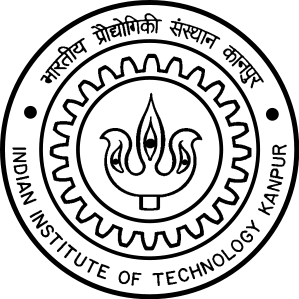
\includegraphics[scale=0.8]{logo.png}}

\label{logo}
\end{figure}
		
\begin{table}[h]
    \centering
    \begin{tabular}{|l|l|l|l|}
        \hline
        \textbf{Member} & \textbf{Roll Number} & \textbf{Email} \\ \hline
        Vinayak S & 233560040 & vinayaks23@iitk.ac.in \\ \hline
    \end{tabular}
    \caption{A table showing members with their details and contributions.}
    \label{tab:members_contribution}
\end{table}

\end{titlepage}

\tableofcontents

\begin{center}
\chapter{Task 1: Problem Statement}
\end{center}
Daniel is a 
security engineer, 
and he has a got a project
for side-channel analysis of
an AES hardware implementation. He has already collected power traces for that
AES implementation with a 128-bit key K and have stored the traces in
$traces\_AES.csv$ file. The first column in the csv file indicates the plaintext, the
second column indicates the ciphertext and rest of the columns indicates the
sample points. Now Daniel has to analyse the power traces and will have to find the
AES key using Correlation Power Analysis (CPA). Help Daniel to perform the CPA
attack.

\section{Given}

The $traces\_AES.csv$ file contains three columns: $Plaintext$, $Ciphertext$, and $Traces$. 
This file represents actual power trace data collected from a power analysis experiment conducted on a chip. 
Each row corresponds to power trace measurements for 10 rounds of AES encryption associated with a specific plaintext-ciphertext pair.

\section{Expectations}

We have to help Daniel in analysing the power traces from the $traces\_AES.csv$ file and recover the entire AES key using Correlation Power Analysis (CPA) attack.

\chapter{Correlation Power Analysis (CPA)}

\section{Theory}

Like in the DoM based DPA attack, the Correlation Power Attack (CPA) also relies on targeting an intermediate computation, typically the input or output of an S-Box. These intermediate values are as seen previously computed from a known value, typically the ciphertext and a portion of the key, which is guessed. The power model is subsequently used to develop a hypothetical power trace of the device for a given input to the cipher. This hypothetical power values are then stored in a matrix for several inputs and can be indexed by the known value of the ciphertext or the guessed key byte. This matrix is denoted as H, the hypothetical power matrix. Along with this, the attacker also observes the actual power traces, and stores them in a matrix for several inputs. The actual power values can be indexed by the known value of the ciphertext and the time instance when the power value was observed. This matrix is denoted as T, the real power matrix. It may be observed that one of the columns of the matrix H corresponds to the actual key, denoted as kc. In order to distinguish the key from the others, the attacker looks for similarity between the columns of the matrix H and those of the matrix T. The similarity is typically computed
using the Pearson’s Correlation coefficient as defined in formula below. 

$$result[i][j] = \frac{\sum_{k=0}^{N_{Sample}} (hPower[i][k] - meanH[i])(trace[j][k] - meanTrace[j])}{\sqrt{\sum_{k=0}^{N_{Sample}} (hPower[i][k] - meanH[i])^2 \sum_{k=0}^{N_{Sample}} (trace[j][k] - meanTrace[j])^2}}$$ \\

or Simplified as \\

$$r = \frac{n \sum xy - (\sum x)(\sum y)}{\sqrt{[n \sum x^2 - (\sum x)^2][n \sum y^2 - (\sum y)^2]}}$$

\chapter{Analysis of Trace data}

\section{Dataset analysis}
The dataset contains 30,000 rows and 152 columns, with two columns containing plaintext and ciphertext, and the remaining columns containing traces of power consumption.

The values in the Traces column are as follows:

\{383, 384, 382, 381, 385, 371, 370, 372, 380, 369, 373, 379, 368, 374, 386, 367, 376, 378, 377, 375, 366, 360, 361, 365, 364, 359, 363, 362, 387, 358, 388, 357, 356, 389, 355, 390, 354, 391, 353, 352, 392, 351, 393, 350, 349, 348, 394, 395, 346, 344

The remaining columns, except for Plaintext and Ciphertext, contain integer values representing power consumption traces.


\section{Reading the dataset}

Let's import the required libraries. The pandas library is required to read the dataset in csv format and create a dataframe. The numpy library is required to make the Mathematical functions. The 
scipy's pearsonr is required to calculate the Pearsons coefficient for two values.\\


\begin{lstlisting}[language=Python, caption=Imports the libraries]

    import pandas as pd
    import numpy as np
    from scipy.stats import pearsonr
    from numpy import unravel_index
\end{lstlisting}

After importing the required libraries , now lets read the dataset, using the below lines of code.\\


\begin{lstlisting}[language=Python, caption=Reading the dataset]
    pd.set_option('display.max_rows', None)
    pd.set_option('display.max_columns', None)
    
    df = pd.read_csv('traces_AES.csv',header=None)
    
    print(df.head().to_markdown(index=False, numalign="left",
    stralign="left"))
    print(df.info())
\end{lstlisting}

\section{Extract Columns}

The columns $traces$ , $Ciphertext$ and $Plaintext$ are extracted in the following code. Unfortunately in the csv file the 0x0 is just a single character we need to format it to take 128bits. Hence we use the function $plaintextformat$ as shown below \\


\begin{lstlisting}[language=Python, caption=Normalising the data]
    def plaintextformat(plaintext):
    if plaintext == '0':
        return '00000000000000000000000000000000'
    else:
        return plaintext
\end{lstlisting} 


\begin{lstlisting}[language=Python, caption=Extracting Columns]
    traces = df.iloc[1:, 2:].values
    plaintexts = df.iloc[1:, 0].values
    formattedplaintext = np.array(
        [plaintextformat(pt) for pt in plaintexts],dtype=object)
    ciphertexts = df.iloc[1:, 1].values
    NSample,NPoint= np.shape(traces)
\end{lstlisting} 

\chapter{Computing Correlation Coefficient for Simulated Power Traces for AES}

To analyze the power consumption of an AES implementation, we simulate its behavior, employing the Hamming Distance model for this example. We collect a set of real power measurements, stored as $$trace[NSample][NPoint]$$ where $NSample$ represents the number of encryption operations and $NPoint$ denotes the timing points of interest. In recorded data $traces\_AES.csv$, $NPoint$ is 150.\\

To create hypothetical power consumption data, the attacker focuses on the final round 
(Round 10) of AES. The attacker aims to recover a specific key byte. To do this, they need to predict the power consumption based on a guess of that key byte and the known ciphertext.\\

The process involves analyzing the transitions that occur in the AES registers during Round 10. Due to the ShiftRows operation within AES, the Hamming Distance calculations must account for the byte reordering. For example, to estimate the power consumption associated with the change in register R1, the attacker needs to compute the Hamming Distance between the state of R1 before and after the final round's SubBytes and key addition.\\

Specifically, the attacker targets a key byte (e.g., `k5`). They know the corresponding ciphertext byte (e.g., `C5`). To calculate the hypothetical power consumption, they perform the following steps:\\

\begin{itemize}
    \item Key Guess: The attacker guesses a value for the key byte `k5`.
    \item Ciphertext Manipulation: They XOR the guessed key byte `k5` with the corresponding ciphertext byte `C5`, creating `SCipher`.
    \item Inverse SubBytes: They apply the Inverse SubBytes operation to the result \\
    (`InverseSBOX[SCipher]`). 
    This step reverses part of the final round transformation, yielding an approximation of the state before the final SubBytes.
    \item Hamming Distance Calculation: They compute the Hamming Distance of the result of XOR between ShiftRow byte and the result of the Inverse SubBytes operation. This Hamming Distance represents the predicted power consumption related to the state transition.
    \item Correlation Analysis: This process is repeated for all possible values of `k5`, generating a set of hypothetical power traces. These hypothetical traces are then compared to the real power traces using correlation analysis. The key guess that yields the highest correlation coefficient is considered the most likely correct value for `k5`.
\end{itemize}

Essentially, the attacker is leveraging the known ciphertext and their key guesses to simulate the power consumption during the final round of AES. By comparing these simulations with the actual power measurements, they can statistically identify the correct key byte.


\section{Helper Objects and Functions}

We need inverse S-Box tuple which is a tuple of hex values that make up the inverse of S-Box (SubBytes). It is defined as follows.\\


\begin{lstlisting}[language=Python, caption=Inverse SBOX tuple]
    InverseSbox = (
    0x52, 0x09, 0x6A, 0xD5, 0x30, 0x36, 0xA5, 0x38, 0xBF, 0x40, 0xA3, 0x9E, 0x81, 0xF3, 0xD7, 0xFB,
    0x7C, 0xE3, 0x39, 0x82, 0x9B, 0x2F, 0xFF, 0x87, 0x34, 0x8E, 0x43, 0x44, 0xC4, 0xDE, 0xE9, 0xCB,
    0x54, 0x7B, 0x94, 0x32, 0xA6, 0xC2, 0x23, 0x3D, 0xEE, 0x4C, 0x95, 0x0B, 0x42, 0xFA, 0xC3, 0x4E,
    0x08, 0x2E, 0xA1, 0x66, 0x28, 0xD9, 0x24, 0xB2, 0x76, 0x5B, 0xA2, 0x49, 0x6D, 0x8B, 0xD1, 0x25,
    0x72, 0xF8, 0xF6, 0x64, 0x86, 0x68, 0x98, 0x16, 0xD4, 0xA4, 0x5C, 0xCC, 0x5D, 0x65, 0xB6, 0x92,
    0x6C, 0x70, 0x48, 0x50, 0xFD, 0xED, 0xB9, 0xDA, 0x5E, 0x15, 0x46, 0x57, 0xA7, 0x8D, 0x9D, 0x84,
    0x90, 0xD8, 0xAB, 0x00, 0x8C, 0xBC, 0xD3, 0x0A, 0xF7, 0xE4, 0x58, 0x05, 0xB8, 0xB3, 0x45, 0x06,
    0xD0, 0x2C, 0x1E, 0x8F, 0xCA, 0x3F, 0x0F, 0x02, 0xC1, 0xAF, 0xBD, 0x03, 0x01, 0x13, 0x8A, 0x6B,
    0x3A, 0x91, 0x11, 0x41, 0x4F, 0x67, 0xDC, 0xEA, 0x97, 0xF2, 0xCF, 0xCE, 0xF0, 0xB4, 0xE6, 0x73,
    0x96, 0xAC, 0x74, 0x22, 0xE7, 0xAD, 0x35, 0x85, 0xE2, 0xF9, 0x37, 0xE8, 0x1C, 0x75, 0xDF, 0x6E,
    0x47, 0xF1, 0x1A, 0x71, 0x1D, 0x29, 0xC5, 0x89, 0x6F, 0xB7, 0x62, 0x0E, 0xAA, 0x18, 0xBE, 0x1B,
    0xFC, 0x56, 0x3E, 0x4B, 0xC6, 0xD2, 0x79, 0x20, 0x9A, 0xDB, 0xC0, 0xFE, 0x78, 0xCD, 0x5A, 0xF4,
    0x1F, 0xDD, 0xA8, 0x33, 0x88, 0x07, 0xC7, 0x31, 0xB1, 0x12, 0x10, 0x59, 0x27, 0x80, 0xEC, 0x5F,
    0x60, 0x51, 0x7F, 0xA9, 0x19, 0xB5, 0x4A, 0x0D, 0x2D, 0xE5, 0x7A, 0x9F, 0x93, 0xC9, 0x9C, 0xEF,
    0xA0, 0xE0, 0x3B, 0x4D, 0xAE, 0x2A, 0xF5, 0xB0, 0xC8, 0xEB, 0xBB, 0x3C, 0x83, 0x53, 0x99, 0x61,
    0x17, 0x2B, 0x04, 0x7E, 0xBA, 0x77, 0xD6, 0x26, 0xE1, 0x69, 0x14, 0x63, 0x55, 0x21, 0x0C, 0x7D,
)
\end{lstlisting} 

\newpage

We also need Hamming Distance Function , which is defined in the following HW function.\\

\begin{lstlisting}[language=Python, caption=Hamming Distance Function]
    def HW(x):
        return bin(x).count('1')
\end{lstlisting}

Let us also define the ShiftRow operation matrix as shown in the figure below which associates the positional change in the registers.\\

\begin{figure}[H]
    \centering
    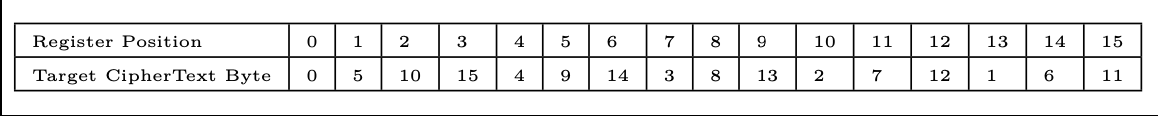
\includegraphics[width=1\linewidth]{image.png}
    \caption{Target Ciphertext Byte wrt. Register Position to Negotiate Inverse Shift
    Row}
    \label{fig:enter-label}
\end{figure}

We need to define a dictonary which maps the 10th round register values to the shift row changes in the 9th round. It is defined below as follows.\\



\begin{lstlisting}[language=Python, caption=dict for the inverse SR ]
    InvSRAdj = {
        0 : 0, 
        1 : 5, 
        2 : 10, 
        3 : 15, 
        4: 4, 
        5: 9, 
        6: 14, 
        7: 3, 
        8: 8, 
        9: 13, 
        10: 2, 
        11: 7, 
        12: 12, 
        13: 1, 
        14: 6, 
        15: 11
    }
\end{lstlisting}

\section{Divide and Conquer attack on the dataset}

The total items (16) in this dictonary also points to our dimensions of 4*4 matrix of AES and all of the operations such as Inv SubBytes and Inv ShiftRows can be defined on this 4*4 matrix. And the entire cipher text of 128bits can be split into 4bytes into this 4*4 matrix. Each element of this matrix is a 4bytes of this cipher text. We can start looping through each element of this matrix and perform our xor with round key from 0x00 to 0xFF and take inverse SBOX and do shift row. Thus by doing this for all elements of this matrix we can create a hypothetical model by using hamming Distance model. We should also loop through the NSample to retrive the ciphertexts. The idea here is to have a divide and conquer rule where we do the operations to find the HYP model byte by byte.\\

\newpage 
\begin{lstlisting}[language=Python, caption=Code Block for divide and conquer ]
hypoModel =  np.empty([NSample, 256],dtype=np.float64)
CorrMatrix = np.empty([256, NPoint], dtype=np.float64)

for row , shiftrow in InvSRAdj.items():
    print(f"Row in process {row} and shiftRow index in consideration {shiftrow}")

    for i in range(NSample):
        for key in range(int('ff',16)+ 1):
            ciphertext = int(ciphertexts[i][row*2:(row*2)+2],16)
            #print(f"Now XORing with ciphertext {hex(ciphertext)} and Key {key}")
            xorwithkey = ciphertext ^ key
            #print(f"XOR result {hex(xorwithkey)}")
            intermediateState = int(InverseSbox[xorwithkey])
            #print(f"output of inv sbox {hex(intermediateState)}")
            outputofSR = int(ciphertexts[i][shiftrow*2:(shiftrow*2)+2],16)
            #print(f"output of SR {hex(outputofSR)}")
            SRxorSB = outputofSR ^ intermediateState
            #print(f"output of xor of SR and SB {SRxorSB}")
            hammingDistance = HW(SRxorSB)
            #print(f"Output after applying HW {hammingDistance}")
            hypoModel[i,key] = hammingDistance
            #print(f"Array of hypoModel = {hypoModel}")

    # Now that we have the hypothetical model, we need to perform CPA that means we have to find
    # co relation co-efficient for each item in the hypothetical model and actual power trace.
    hypoModelDF = pd.DataFrame(hypoModel,dtype=np.float64)
    #hyprows, hypcolumns = hypoModelDF.shape
    #print(f"Rows: {hyprows}, Columns: {hypcolumns}")
    #print(hypoModelDF)
    traceDF = pd.DataFrame(traces,dtype=np.float64)
    #rows, columns = traceDF.shape
    #print(f"Rows: {rows}, Columns: {columns}")
    for i in range(256):
        for j in range(NPoint):
            corr1 = hypoModelDF.iloc[:, i].values
            corr2 = traceDF.iloc[:, j].values
            corr, _ = pearsonr(corr1, corr2)
            CorrMatrix[i, j] = abs(corr)       
    x, y = unravel_index(CorrMatrix.argmax(), CorrMatrix.shape)
    print(f"The key byte value with the highest correlation is",x,"the key byte value in hex is ",hex(x))
\end{lstlisting}
\newpage 
Upon executing this code block cell which basically iterates over each element of the trace and the each element of the hypothetical model obtained from the previous cell block and retrives the correlation index for these two values and the element with the highest corelation is guessed as the key byte and key in hex as shown below.
\lstset{%
  language={[latex]TeX},
  tabsize=2,
  breaklines,
  basicstyle=\footnotesize\ttfamily,
}
\begin{lstlisting}
Row in process 0 and shiftRow index in consideration 0
The key byte value with the highest correlation is 208 the key byte value in hex is  0xd0
Row in process 1 and shiftRow index in consideration 5
The key byte value with the highest correlation is 20 the key byte value in hex is  0x14
Row in process 2 and shiftRow index in consideration 10
The key byte value with the highest correlation is 249 the key byte value in hex is  0xf9
Row in process 3 and shiftRow index in consideration 15
The key byte value with the highest correlation is 168 the key byte value in hex is  0xa8
Row in process 4 and shiftRow index in consideration 4
The key byte value with the highest correlation is 201 the key byte value in hex is  0xc9
Row in process 5 and shiftRow index in consideration 9
The key byte value with the highest correlation is 238 the key byte value in hex is  0xee
Row in process 6 and shiftRow index in consideration 14
The key byte value with the highest correlation is 37 the key byte value in hex is  0x25
Row in process 7 and shiftRow index in consideration 3
The key byte value with the highest correlation is 137 the key byte value in hex is  0x89
Row in process 8 and shiftRow index in consideration 8
The key byte value with the highest correlation is 225 the key byte value in hex is  0xe1
Row in process 9 and shiftRow index in consideration 13
The key byte value with the highest correlation is 63 the key byte value in hex is  0x3f
Row in process 10 and shiftRow index in consideration 2
The key byte value with the highest correlation is 12 the key byte value in hex is  0xc
Row in process 11 and shiftRow index in consideration 7
The key byte value with the highest correlation is 200 the key byte value in hex is  0xc8
Row in process 12 and shiftRow index in consideration 12
The key byte value with the highest correlation is 182 the key byte value in hex is  0xb6
Row in process 13 and shiftRow index in consideration 1
The key byte value with the highest correlation is 99 the key byte value in hex is  0x63
Row in process 14 and shiftRow index in consideration 6
The key byte value with the highest correlation is 12 the key byte value in hex is  0xc
Row in process 15 and shiftRow index in consideration 11
The key byte value with the highest correlation is 166 the key byte value in hex is  0xa6    
\end{lstlisting}

Thus after performing the Divide and Conquer attack on the dataset we have obtained the 128bit key of the AES ecryption used in the hardware. They obtained was

$$AES_k: d014f9a8c9ee2589e13f0cc8b6630ca6$$

\chapter{Conclusion}

By gathering power traces from AES rounds, along with the associated plaintext and ciphertext pairs, we can link the power consumption to a theoretical model, such as Hamming Distance. This allows us to identify the key byte that exhibits the strongest correlation with the measured power consumption. \\ 
\end{document}
